\documentclass{beamer}
\usepackage{beamerthemesplit}

\usetheme{CambridgeUS}
\usecolortheme{dolphin}
\usepackage{sidecap}
\usepackage[utf8]{inputenc}
\usepackage[frenchb]{babel}



\title{Scientific Computing}
\subtitle {Understanding and solving stochastic PDE }
\author{USHAKOVA Oxana}
\date{\today}
\begin{document}
\maketitle
\tableofcontents


\section{Finance} 
\frame{\frametitle{Notations }

\begin{itemize}
\item $S$ - Stock price, also called Spot price (or any underlying asset)
\item $V(S,t)$ - value of an option, depending on time and spot price
\item $K$ - Strike price
\item $r$ - risk-free rate
\item $d$ - dividend yield
\item $\mu$ - drift rate of $S$ - the rate at which the average of $S$ changes
\item $\sigma$ - volatility of the stock, standard deviation of $log(S)$ - return on stock
\item $T_0$,$T$ - initial and final time
\item $\theta$ - long variance : as $t$ tends to infinity, the expected value of $\nu$ tends to $\theta$ 
\item $\kappa$ - the rate at which $\nu$ reverts to $\theta$
\item $\xi$ - the volatility of volatility
\end{itemize}
}

\frame{\frametitle{Financial mathematics}
\begin{figure}[H]
    \centering
    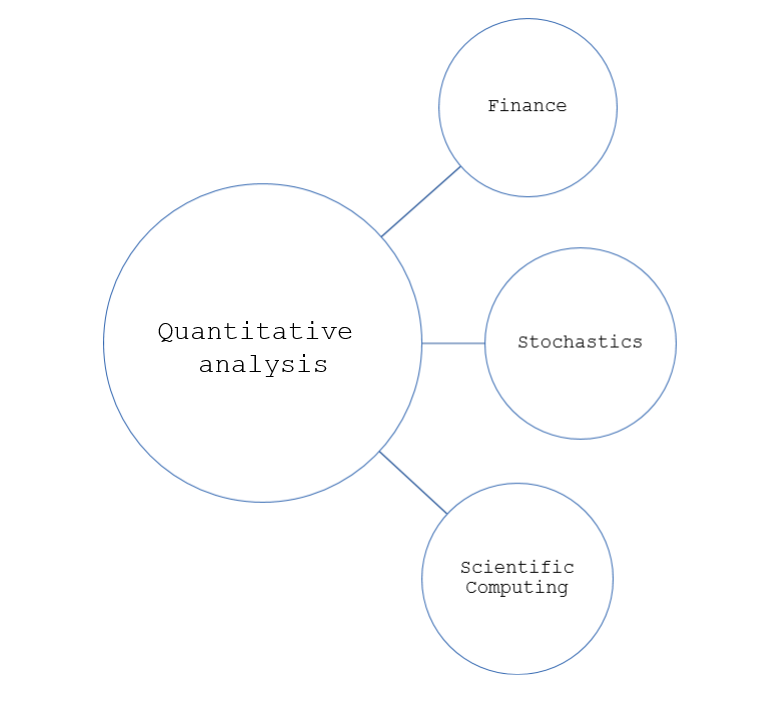
\includegraphics[width=0.5\textwidth]{dia.png}
    \caption{Financial mathematics}
\end{figure}
}




\subsection{Options}




\frame{\frametitle{What is an option ? }

An option - a contract that gives the buyer the right, \textbf{ but not the obligation}, to buy or sell an underlying asset (a stock, a bond, gold, other option) at a specific price, called Strike price, on a certain date, called maturity. \\
\newline
What right is proposed ?
\begin{itemize}
\item The right to buy – \textbf{Call} option
\item The right to sell – \textbf{Put} option
\end{itemize}
}






\frame{\frametitle{What are option parameters? }
Parameters to fix at $t_0$ :
\begin{itemize}
\item Who buys (long), who sells (short)?
\item What is the underlying asset ?
\item What is the maturity $T$ of the contract ?
\item Does the contract give the right to buy (\textbf{call option}) or to sell(\textbf{put option}) ?
\item What is the Strike price $K$ ?
\item What is the price of the option itself, i.e. premium?
\end{itemize}
}




\frame{\frametitle{Long Call Payoff}
\begin{figure}[H]
    \centering
    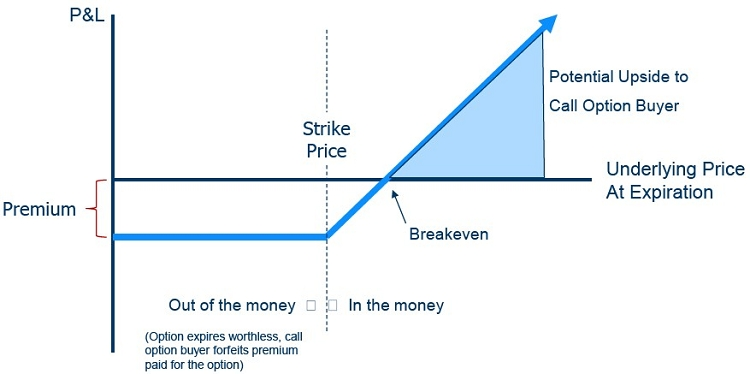
\includegraphics[width=0.5\textwidth]{payoff.png}
    \caption{Options Payoffs}

\end{figure}
Buying Call Option brings profit (\textit{in the money»}), if $S$ at maturity $T$ is higher than the Breakeven point. So the payoff of this option is:  (premium ignored):
\[
 Payoff = 
  \begin{cases} 
   S - K & \text{if } S(T)>K \\
   0       & \text{if not } 
  \end{cases}
\]
}





\frame{\frametitle{Other Payoffs}
\begin{figure}[H]
    \centering
    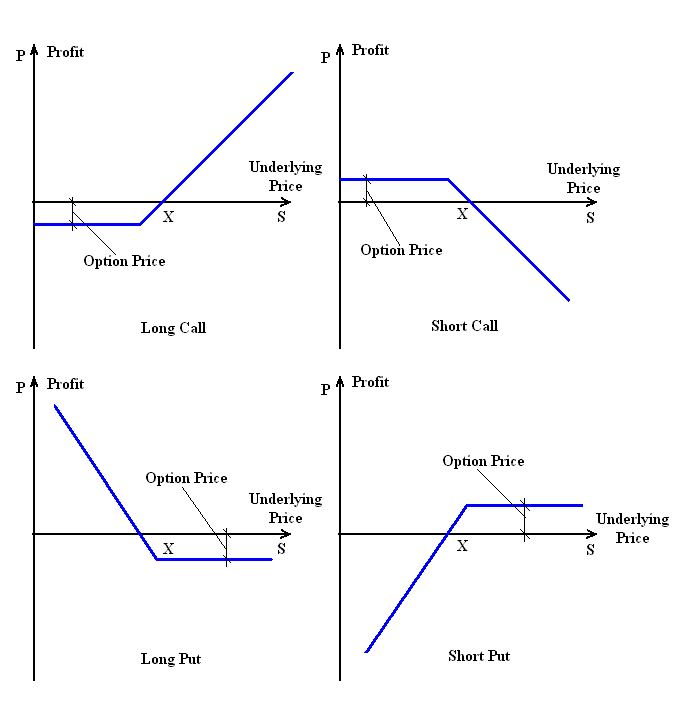
\includegraphics[width=0.5\textwidth]{OptionsProfit.png}
    \caption{Other Payoffs}
\end{figure}
}

\frame{\frametitle{Vanilla VS Exotics }
\textbf{Vanilla Option}\\
\begin{itemize}
\item European option
\end{itemize}
\textbf{Exotic Option}\\
\begin{itemize}
\item American option (Bermudian)
\item Barrier option (Paris)
\item Asian option
\item Lookback option (Russian)
\item Binary option
\item Cliquer option
\item etc, etc..
\end{itemize}
}



\subsection{Greeks}
\frame{\frametitle{Greeks}


\item \textbf{Delta} - the rate of change of the option price w.r.t. the price of the underlying asset: $\delta = \frac{\partial C}{\partial S}$
\item \textbf{Gamma} - the rate of change of the $\delta$ w.r.t. the price of the underlying asset: $\Gamma = \frac{\partial^2 \Pi}{\partial S^2}$ 
\item \textbf{Theta} - the rate of change of the portfolio price w.r.t. the time: $\theta = \frac{\partial \Pi}{\partial t}$
\item \textbf{Vega} - the rate of change of the portfolio price w.r.t. the volatility of the underlying asset: $\upsilon = \frac{\partial \Pi}{\partial \sigma}$
\item \textbf{Rho} - the rate of change of the portfolio price w.r.t. the interest rate:$\upsilon = \frac{\partial \Pi}{\partial r}$
}








\subsection{Pricing Models}

\frame{\frametitle{Pricing models }
\begin{figure}[H]
    \centering
    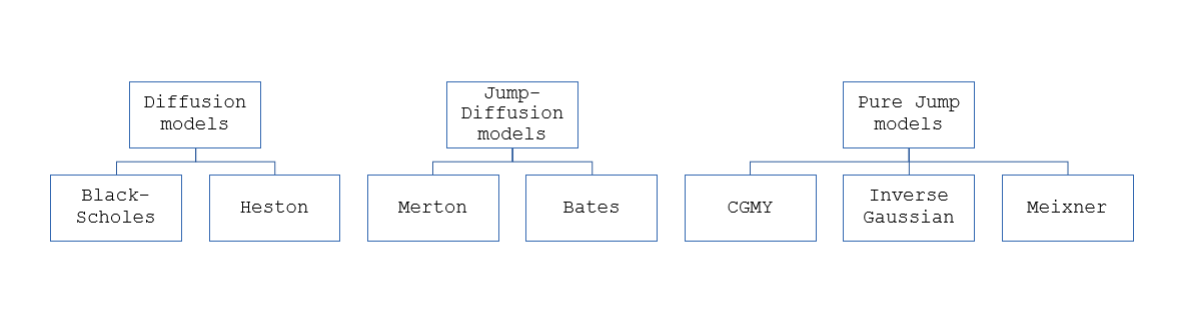
\includegraphics[width=\textwidth]{models.png}
\end{figure}

\begin{figure}[H]
    \centering
    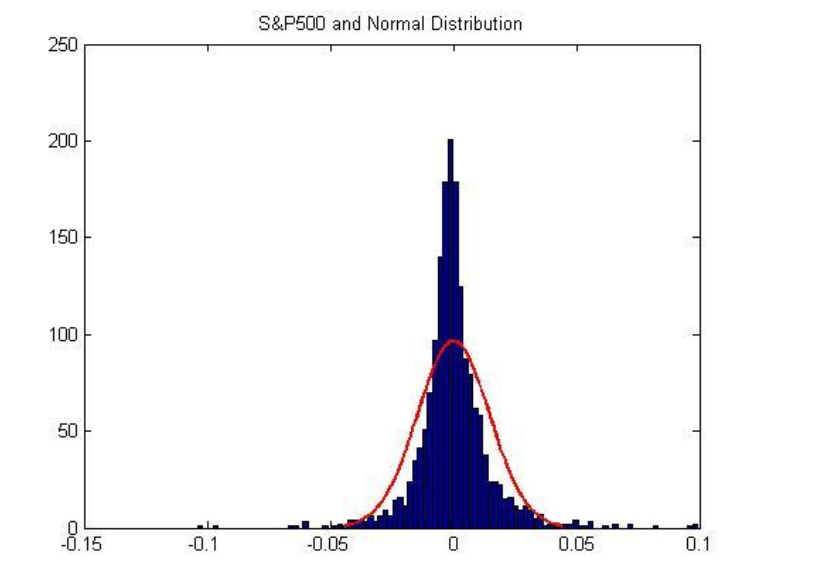
\includegraphics[width=0.4\textwidth]{sp500.png}
\end{figure}
}





\section{Stochastic} 
\subsection{Wiener Process}



\frame{\frametitle{What is a Wiener process}

\begin{itemize}
\item Lévy processes: independent, stationary increments
\item Markov processes: "memoryless"\\
\end{itemize}
\begin{figure}[H]
    \centering
    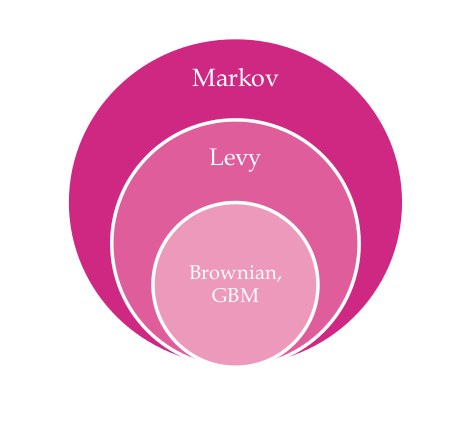
\includegraphics[width=0.4\textwidth]{gbm.png}
\end{figure}



\textbf{BUT}: no jumps ? $\rightarrow$ add Compound Poisson process!
 }




\frame{
\begin{figure}[H]
    \centering
    \caption{Wiener and Wiener-Poisson process}
    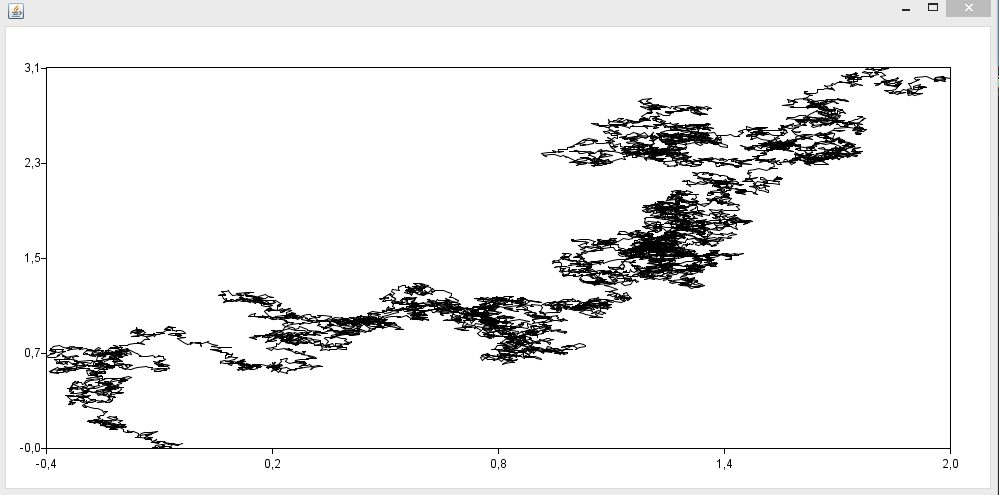
\includegraphics[width=0.55\textwidth]{brown.png}
\end{figure}

\begin{figure}[H]
    \centering
    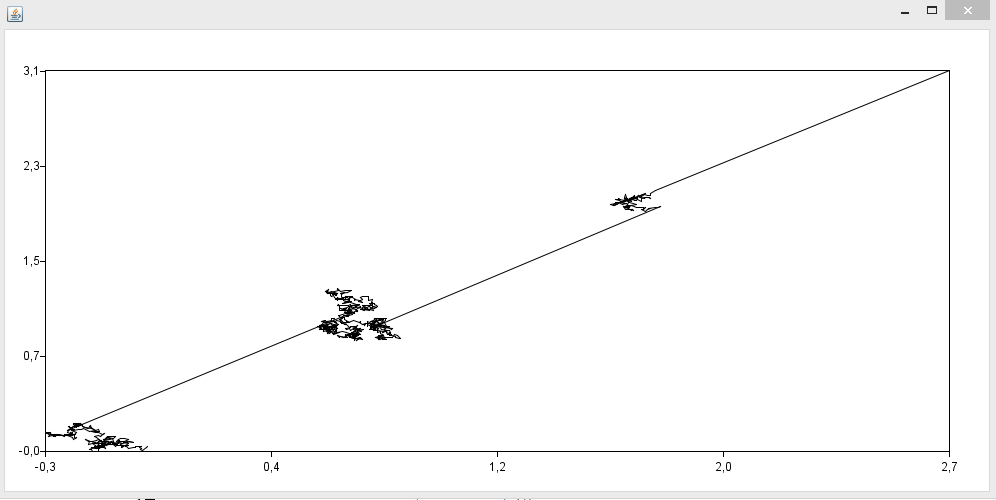
\includegraphics[width=0.55\textwidth]{poisson.png}
\end{figure}
}



\frame{
\begin{figure}[H]
    \centering
    \caption{Black Scholes and Merton}
    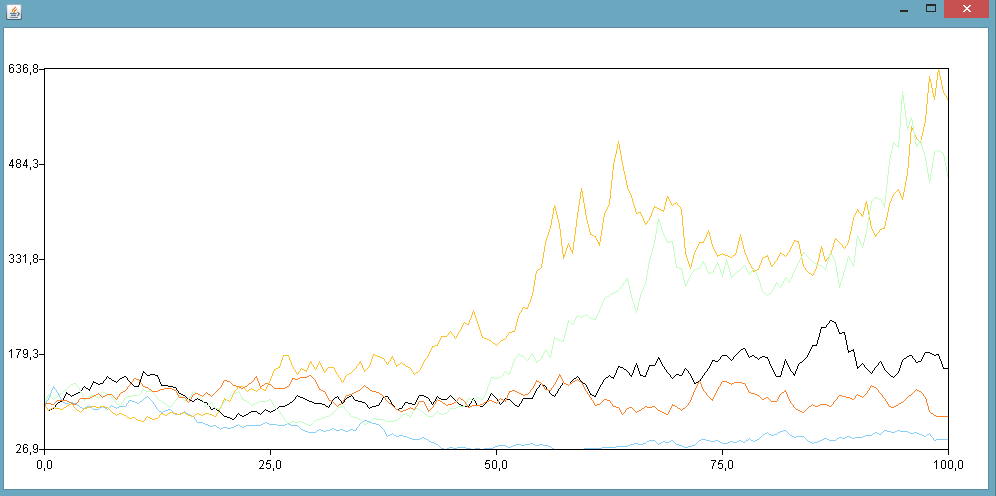
\includegraphics[width=0.55\textwidth]{wiener.png}
\end{figure}

\begin{figure}[H]
    \centering
    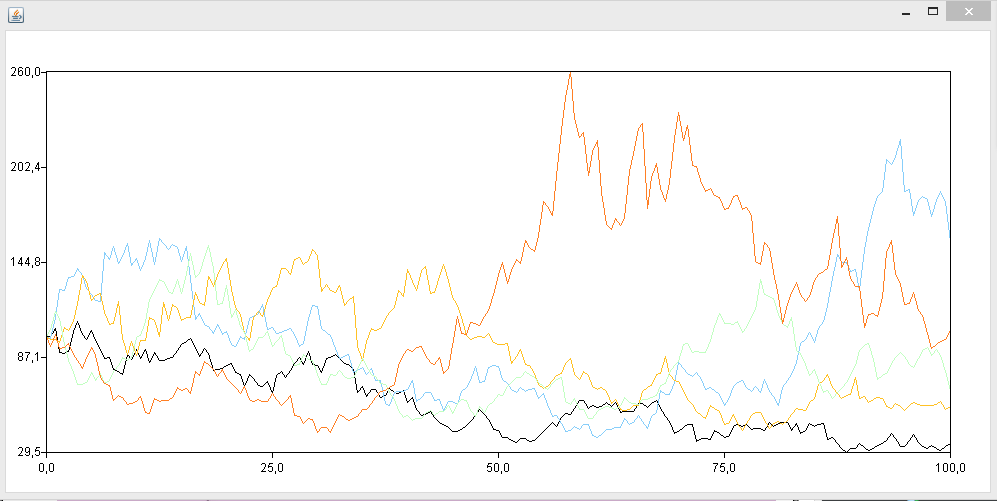
\includegraphics[width=0.55\textwidth]{merton.png}
\end{figure}
}








\subsection{Ito Calculus}

\frame{\frametitle{Ito's lemma and Black-Scholes}
\textbf{Ito's lemma} :

$X_t$  given by: $dX_t = udt+vdB_t$, $f(t,x) \in C^2$, $Y_t=f(t,X_t)$ .

\begin{equation}
dY_t=\frac{\partial f}{\partial t}(t,X_t)dt + \frac{\partial f}{\partial x}(t,X_t)dB_t + \frac{1}{2} \frac{\partial^2 f}{\partial x^2}(t,X_t)(dB_t)^2
\end{equation}

\textbf{Applying to Black-Scholes}:

\begin{equation}
dS_t=\mu S_t dt + \sigma S_t dB_t, X_0>0
\end{equation}
with $f(t,x)=ln x$,$f \in C^2$ and  $Y_t = ln S_t$, gives:
\begin{equation}
\int_0^T dY_t =(\mu - \frac{1}{2} \sigma^2)T + \sigma B_t 
\end{equation}
Or
\begin{equation}
S_T = e^{Y_T}=S_0 e^{(\mu - \frac{1}{2} \sigma^2)T+\sigma dB_t }
\end{equation}

}



\section{Black-Scholes equation} 
\subsection{Overview}

\frame{\frametitle{Technical aspects}
\begin{itemize}
\item Derivation
\begin{itemize}
\item Economic approach
\item From Heat PDE
\end{itemize}
\end{itemize}
\begin{itemize}
\item Numerical methods:
\begin{itemize}
\item Monte-Carlo (Box-Muller Algorithm)
\item Tree methods (Cox-Ross-Rubenstein model)
\item \textbf{Solving PDE}
\end{itemize}
\item $S_t$ follows Geometric Brownian motion:
$dS_t = S_t \mu dt+S_t \sigma dB_t$
\item Put-Call Parity:
\begin{equation}
C + Ke^{-rT} = P + S_0
\end{equation}
\end{itemize}
}



\frame{\frametitle{Why use the Geometric Brownian motion?}

\begin{itemize}
\item The expected returns of GBM are independent of the value of the process (stock price), which agrees with what we would expect in reality.
\item A GBM process only assumes positive values, just like real stock prices.
\item A GBM process shows the same kind of 'roughness' in its paths as we see in real stock prices.
\item Calculations with GBM processes are relatively easy.
\end{itemize}
}

\frame{\frametitle{GBM path in C++ with gnuplot}
\begin{figure}[H]
    \centering
    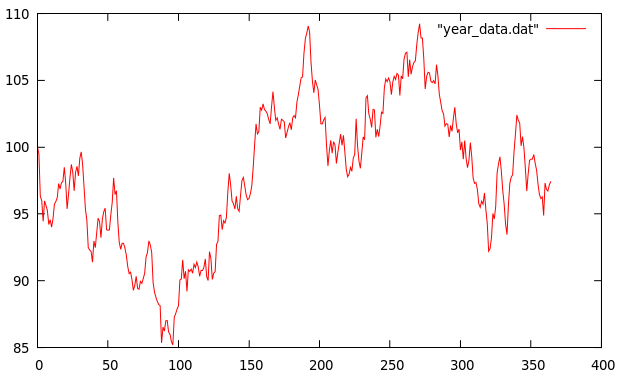
\includegraphics[width=0.8\textwidth]{gbmgnu.png}
    \caption{GBM path}
\end{figure}   
}


\frame{\frametitle{Black-Scholes analytical solution}
With Ito's lemma we find : 
\begin{equation}
S_T = e^{Y_T}=e^{Y_0+(\mu - \frac{1}{2} \sigma^2)T+\sigma dB_t}=S_0 e^{(\mu - \frac{1}{2} \sigma^2)T+\sigma dB_t }
\end{equation}
and


\begin{equation}
C = e^{-dT}S_0 \mathcal{N}(d_1)-e^{-rT}K\mathcal{N}(d_2))
\end{equation}
\begin{equation}
P = e^{-rT}K\mathcal{N}(-d_2))-e^{-dT}S_0 \mathcal{N}(-d_1)
\end{equation}
with \\

$ d_1 =\frac{ \ln (\frac{S_0}{K}) + (r-d + \frac{\sigma^2}{2} )T}{\sigma \sqrt{T}} $ \\

$ d_2 = \frac{\ln (\frac{S_0}{K}) + (r-d - \frac{\sigma^2}{2} )T}{\sigma \sqrt{T}}  = d_1 -\sigma \sqrt{T} $ 
}


\section{Finite Element Method} 
\subsection{Overview}


\frame{\frametitle{Black-Scholes PDE - Call and Put }
\begin{equation}
\frac{\partial C}{\partial t}+\frac{1}{2} \sigma^2 S^2\frac{\partial^2 C}{\partial S(t)^2} + rS(t)\frac{\partial C}{\partial S(t)} - rC=0
\end{equation}
$C(0,t)=0$\\
$C(S,t) = e^{-dT}S_0-e^{-rT}K$ when $S$\longrightarrow $\infty$ \\
$C(S,T) = max(S-K,0)$
\begin{equation}
\frac{\partial P}{\partial t}-\frac{1}{2} \sigma^2 S^2\frac{\partial^2 P}{\partial S(t)^2} - rS(t)\frac{\partial P}{\partial S(t)} + rP=0
\end{equation}
$P(0,t) =e^{-rT}K$\\
$P(S,t) = 0 $ when $S$\longrightarrow \infty \\
$P(S,T) = max(K-S,0)$
}

\frame{\frametitle{Black-Scholes PDE terms }
\begin{equation}
\frac{\partial C}{\partial t}+\frac{1}{2} \sigma^2 S^2\frac{\partial^2 C}{\partial S(t)^2} + rS(t)\frac{\partial C}{\partial S(t)} - rC=0
\end{equation}

\begin{itemize}
\item Diffusion term: $\frac{1}{2} \sigma^2 S^2\frac{\partial^2 C}{\partial S(t)^2}$ 
\item Convection term: $ rS(t)\frac{\partial C}{\partial S(t)}$
\end{itemize}

Peclet number : $\frac{diff}{conv}=\frac{rS}{\frac{1}{2} \sigma^2 S^2}=\frac{2rS}{\sigma^2 S^2}=\frac{2r}{\sigma^2 S}$\\
\textbf{Remarque} :  $Pe<\frac{r}{\sigma^2}$, if not, then small $\sigma$ is not compensated by a small $r$.
}
\frame {\frametitle{Weak Formulation}
Linear parabolic PDE with non-constant coefficients and non-homogenous boundary conditions and, possibly, non-differentiable or discontinuous final conditions:
\begin{itemize}
\item Choosing space : Weighted Sobolev $ \forall u \in V,  V=\{ v \in L^2(\mathbb{R}_+) : S\frac{\partial v}{\partial S} \in L^2(\mathbb{R}_+) \}$
\item Bilinear form $a$:
\begin{equation}
a(u,w)=\int_0^\infty \frac{\partial u}{\partial S} \frac{\sigma^2}{2} \frac{S^2w}{\partial S} - rSw\frac{\partial u}{\partial S} + ruw
\end{equation}
\item Weak formulation (for put):
\begin{equation}
(\frac{\partial u}{\partial t}, w) + a(u,w) = 0, \forall w \in V
\end{equation}
\end{itemize}
}
\frame {\frametitle{Existence and Uniqueness}
Martingales + Filtration + Ito Calculus
 
\begin{figure}[H]
    \centering
    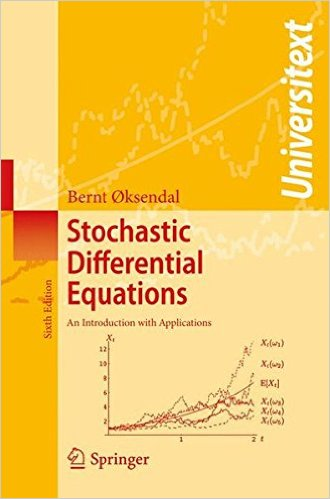
\includegraphics[width=0.3\textwidth]{Oks.jpg}
    \caption{Oksendal - SDE (6ed)}
\end{figure}   
}

\frame{\frametitle{Mesh adaptation and Delaunay Triangulation }
Delanay algorithm: interpolation error is bounded by:
\begin{equation}
||u-u_h||<C|| \nabla ( \nabla u)h^2
\end{equation}
\begin{itemize}
\item no obtuse triangles
\item neighbour triangles with the same size
\end{itemize}
For each edge the circle circumscribing one triangle does not contain the fourth vertex.
\begin{figure}[H]
    \centering
    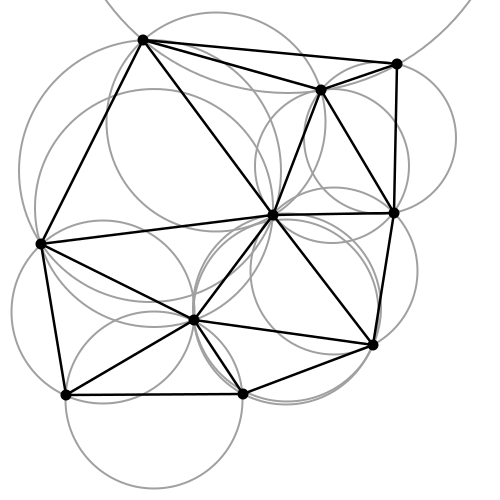
\includegraphics[width=0.3\textwidth]{Delaunay.png}
    \caption{Delaunay Triangulation}

\end{figure}
}


\subsection{Numerical Results}


\frame{\frametitle{Vanilla put}

\begin{figure}[H]
   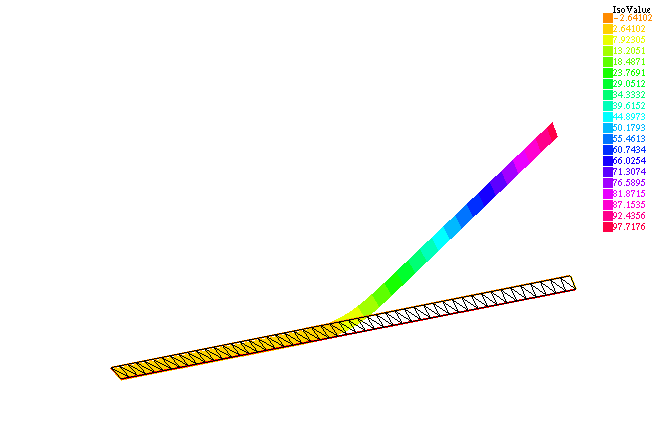
\includegraphics[width=0.475\textwidth]{s01.png}
   \hfill
   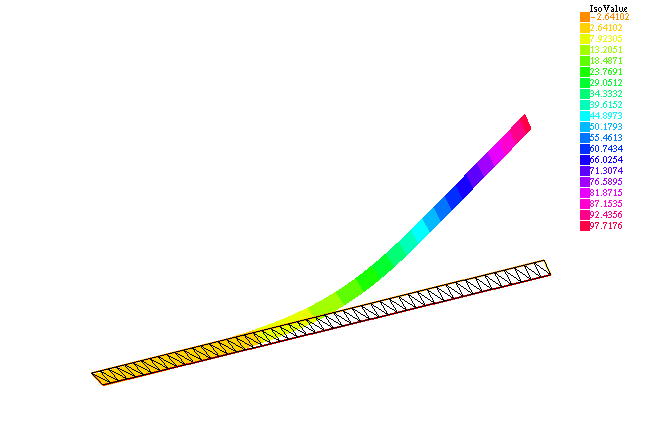
\includegraphics[width=0.475\textwidth]{s03.png}
    \caption{ $\sigma=0.1$ and $\sigma=0.3$}
\end{figure}
}



\frame{\frametitle{Barrier put : 30, 90, 100 with K=100}
\begin{figure}[H]
   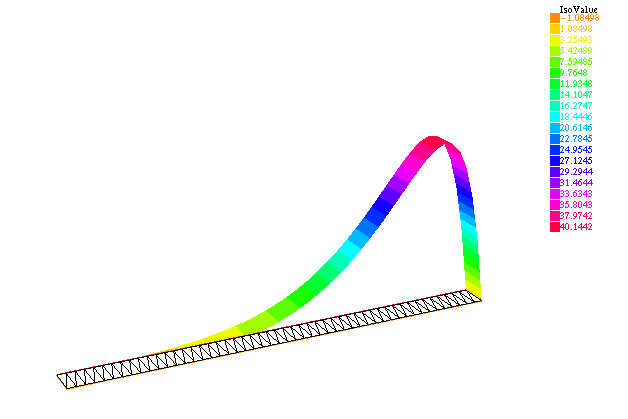
\includegraphics[width=0.300\textwidth]{b30.png}
   \hfill
   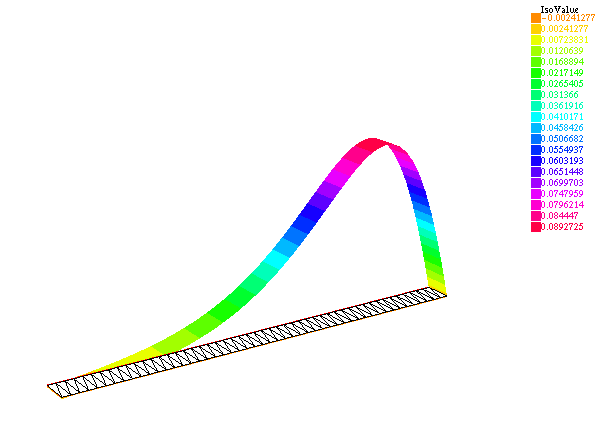
\includegraphics[width=0.300\textwidth]{b90.png}
	\hfill   
   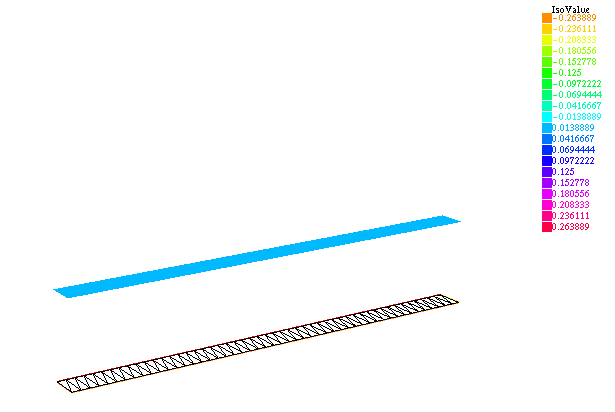
\includegraphics[width=0.300\textwidth]{b100.png}
    \caption{ barriers = $30,90,100$}
\end{figure}
}


\frame{\frametitle{Delta and Gamma for $\sigma$ = 0.1, 0.3 }
\begin{figure}[H]
    \centering
    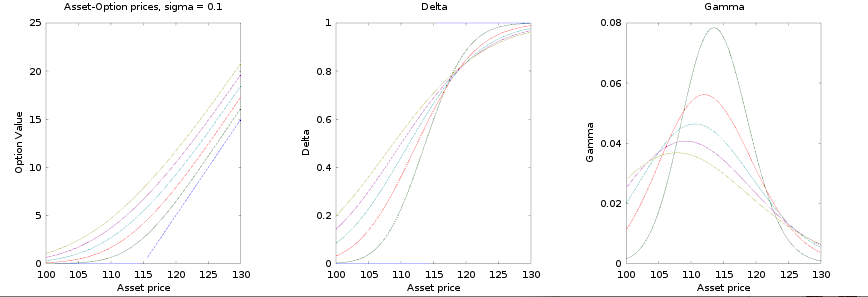
\includegraphics[width=0.83\textwidth]{octave1.png}
\end{figure}

\begin{figure}[H]
    \centering
    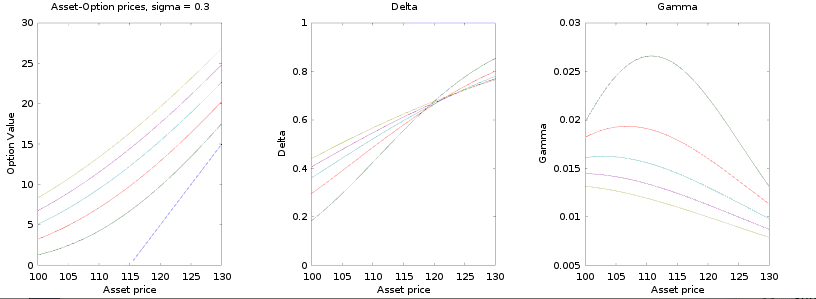
\includegraphics[width=0.83\textwidth]{octave2.png}
\end{figure}
}






\frame{\frametitle{Delta for $\sigma$ = 0.1 }


\begin{figure}[H]
   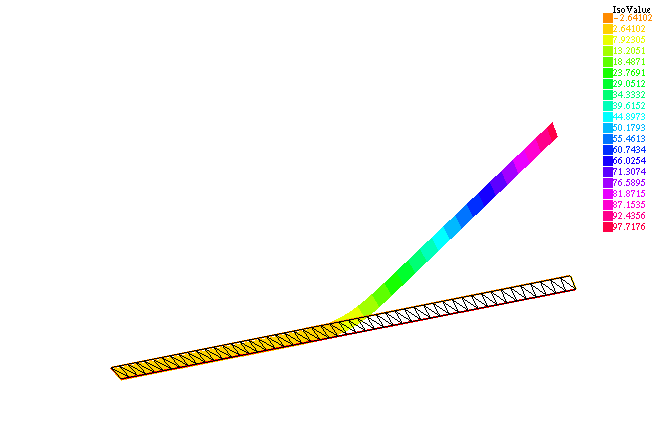
\includegraphics[width=0.475\textwidth]{s01.png}
   \hfill
   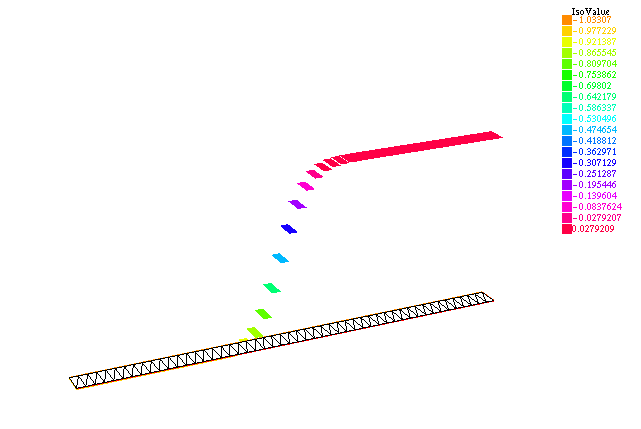
\includegraphics[width=0.475\textwidth]{d01.png}
    \caption{ $\sigma=0.1$ and $\sigma=0.3$}
\end{figure}
}

\frame{\frametitle{Delta for $\sigma$ = 0.3 }

\begin{figure}[H]
   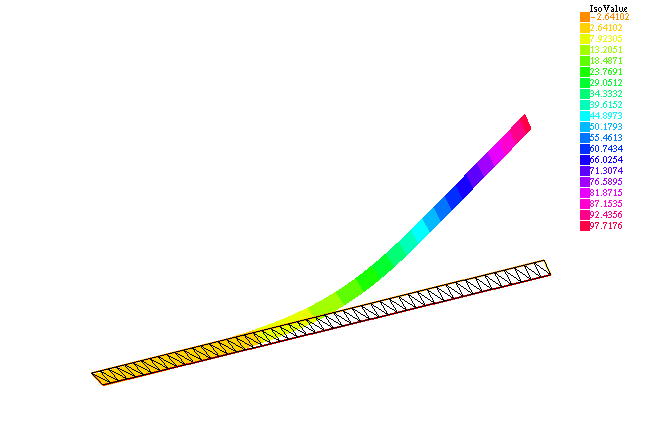
\includegraphics[width=0.475\textwidth]{s03.png}
   \hfill
   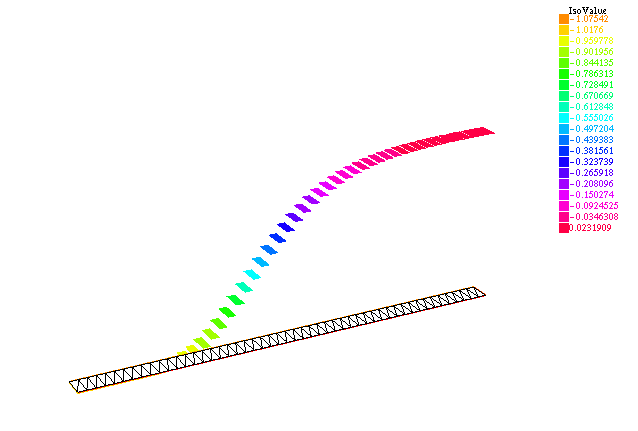
\includegraphics[width=0.475\textwidth]{d03.png}
    \caption{ Delta for $\sigma=0.1$ and $\sigma=0.3$}
\end{figure}
}







\frame{\frametitle{Vanilla 2D}
Classic asymmetric data
\begin{figure}
   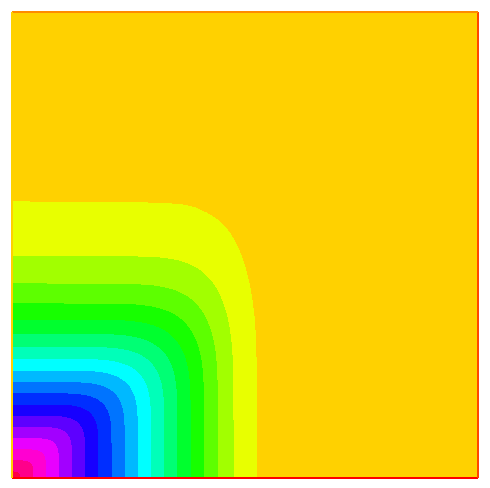
\includegraphics[width=0.475\textwidth]{bs1a.png}
   \hfill
   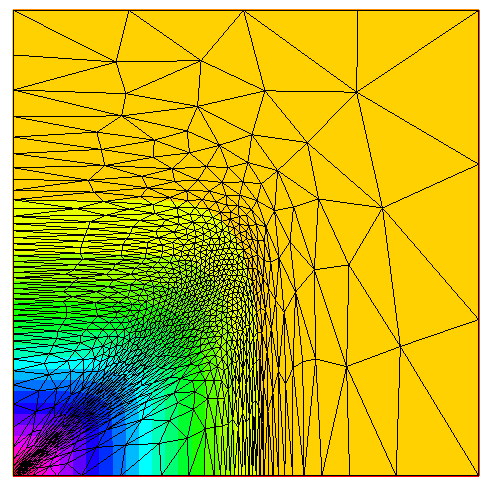
\includegraphics[width=0.475\textwidth]{bs1b.png}
\end{figure}
}


\frame{\frametitle{Vanilla 2D}
Low volatility with high correlation
\begin{figure}
   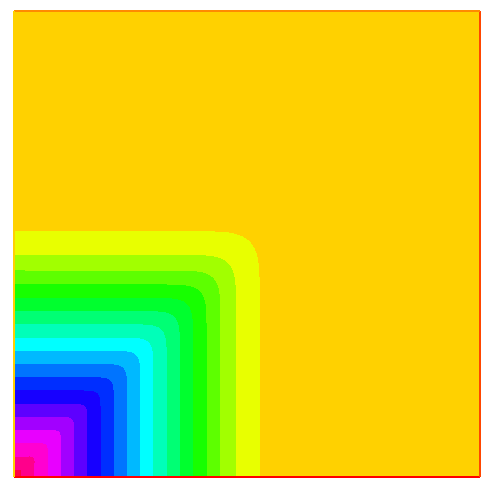
\includegraphics[width=0.475\textwidth]{bs2a.png}
   \hfill
   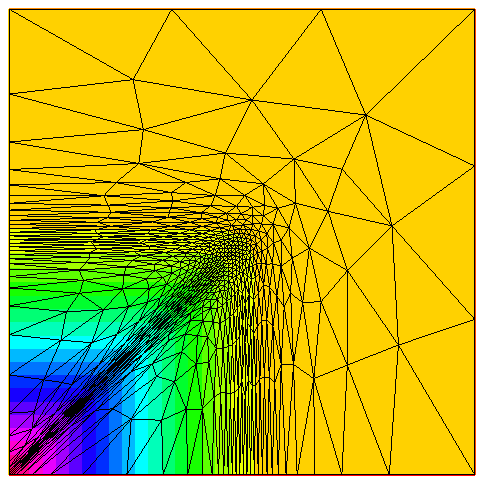
\includegraphics[width=0.475\textwidth]{bs2b.png}
\end{figure}
}


\frame{\frametitle{Vanilla 2D}
High volatility but low correlation
\begin{figure}
   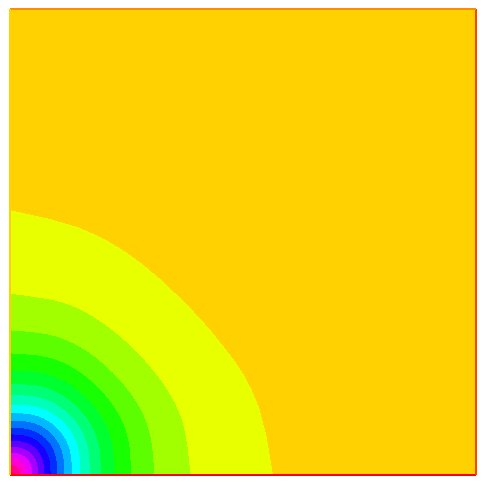
\includegraphics[width=0.475\textwidth]{bs3a.png}
   \hfill
   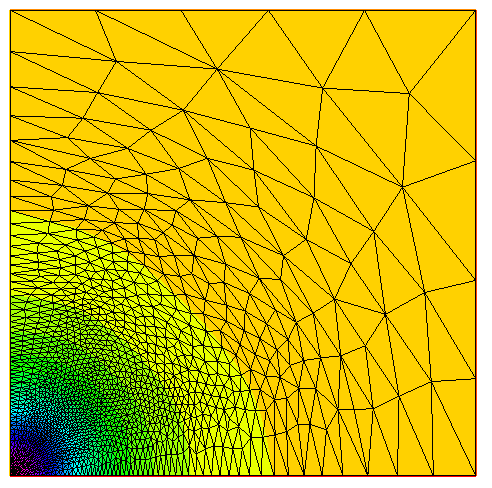
\includegraphics[width=0.475\textwidth]{bs3b.png}
\end{figure}
}


\frame{\frametitle{Vanilla 2D}
High volatility with high correlation
\begin{figure}
   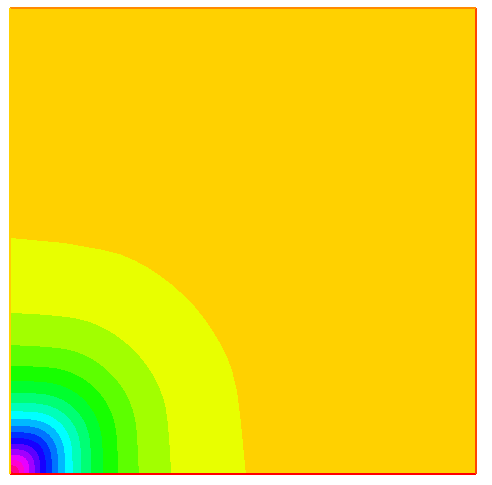
\includegraphics[width=0.475\textwidth]{bs4a.png}
   \hfill
   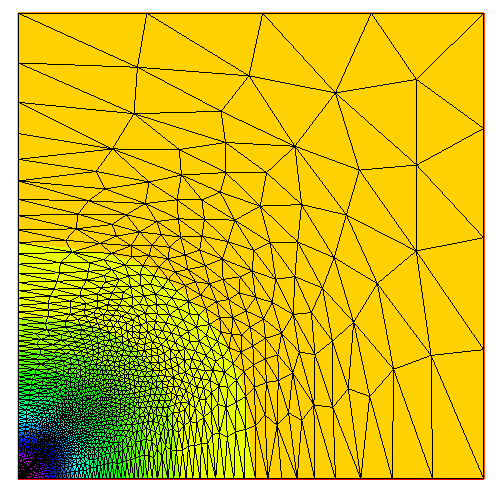
\includegraphics[width=0.475\textwidth]{bs4b.png}
\end{figure}
}

\section{Finite Difference Method}
\subsection{Overview}
\frame{\frametitle{Basics}
\begin{itemize}
\item Forward-Time Central-Space (FTCS) or \textbf{Explicit}
\item Backward-Time Central-Space (BTCS)or Implicit
\item Central-Time Central-Space (CTCS) or Crank-Nicolson 
\end{itemize}

\begin{equation}
V_j^i = \frac{1}{1+r\Delta t}(AV_{j+1}^{i+1}+BV_j^{i+1}+CV_{j-1}^{i+1})
\end{equation}
with 
\begin{itemize}
\item $A=(\frac{1}{2} \sigma^2 j^2+\frac{1}{2} rj)\Delta t $
\item $B=1-\sigma^2 j^2 \Delta t $
\item $C = (\frac{1}{2} \sigma^2 j^2 - \frac{1}{2}rj)\Delta t$
\end{itemize}
}


\frame{\frametitle{"Explicit" grid}
\begin{itemize}
\item Space interval $[0,S^U]$ in $jmax$ intervals of length $\Delta S = S^U/jmax$ 
\item Time interval $[0,T]$ in $imax$ intervals of length $\Delta t = T/imax$\\
\item The value at each node $V(j\Delta S, i \Delta t)$ $\longrightarrow$ $V^i_j$
\end{itemize}


\begin{figure}[H]
   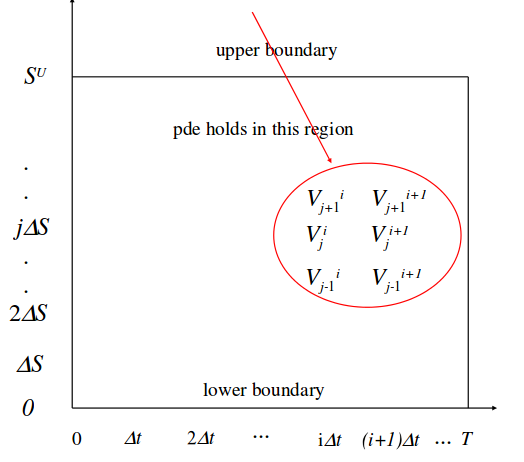
\includegraphics[width=0.5\textwidth]{grid1.png}

\end{figure}

}

\frame{\frametitle{Stability}
Explicit method $\Rightarrow$ unstable ! \\
Conditions of stability derived by using probabilistic approach.\\
If $A,B,C$ as probabilities $\Rightarrow$ positive. 
\begin{itemize}
\item $A$ and $C$ $\rightarrow  j > |\frac{r}{\sigma^2}|$  
\item $B \rightarrow \Delta t < \frac{1}{\sigma^2 j^2}$
\end{itemize} 
Increase $jmax$ by 10 $\rightarrow$ Increase $imax$ by 100.
}

\subsection{Numerical results}
\frame{\frametitle{FDM and Analytical solutions in C++}
\begin{figure}[H]
   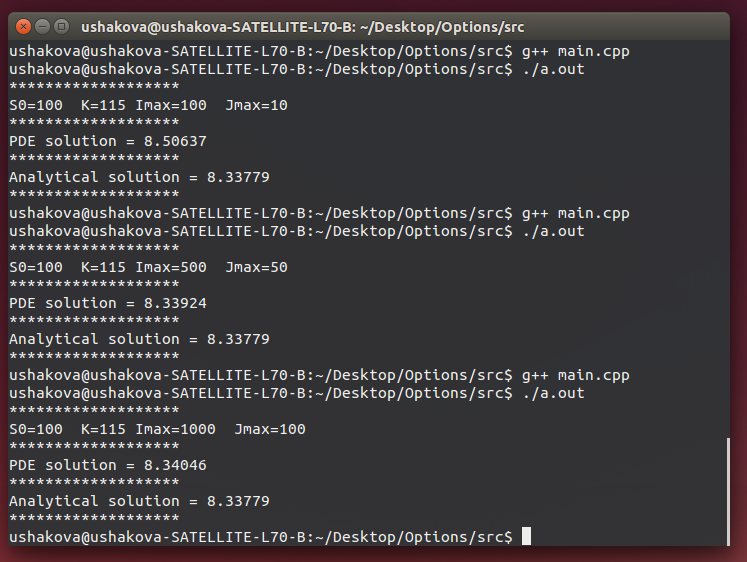
\includegraphics[width=0.7\textwidth]{fdm.png}
    \caption{ FDM and Analytical solutions}
\end{figure}
}

\section{FDM and FEM}
\frame{\frametitle{Comparing FDM and FEM for SDE}
\begin{itemize}
\item Why use FEM?
\begin{itemize}
\item Much more accurate 
\item Lots of free libraries
\end{itemize}
\item Why use FDM?
\begin{itemize}
\item No usual boundary problems
\item Easier to implement
\end{itemize}
\end{itemize}
Further research : Jump-Diffusion models, more complex options, portfolios, Feel++. 
}
\section{Application}
\frame{\frametitle{Importance of accurate pricing and regulation}
\begin{itemize}
\item  FOREX : $\alpha$ - stable processes
\item  Mortgage crisis : NINJA "put" options on houses
\item  Financial crisis : Collateralized Debt Obligation
\item  EU crisis : Greece and Lehman Brothers
\item Biggest losses by banks :CB1965(8 billion USD), SG2008(7 billion USD), etc,etc..
\end{itemize}
}
\section*{The end}
\frame{
\begin{figure}[H]
    \centering
    
\includegraphics[width=\textwidth]{1.png}
\end{figure}   
}

\end{document}
